\section{Auswertung}
\label{sec:Auswertung}

%Tabelle mit Messdaten
%Es folgt eine Tabelle mit den aufgenommenen Messdaten.
%\begin{table}[H]
%  \centering
%  \caption{Veränderung der Reservoirtemperaturen und -drücke sowie der Leistung im Messverlauf.}
%  \label{tab:Messdaten}
%  \sisetup{table-format=2.1}
%  \begin{tabular}{S[table-format=2.0] S S S S S[table-format=3.0]}
%    \toprule
%    {$t \mathbin{/} \unit{\minute}$} 
%    & {$T_1 \mathbin{/} \unit{\celsius}$} & {$T_2 \mathbin{/} \unit{\celsius}$} 
%    & {$p_b \mathbin{/} \unit{\bar}$} & {$p_a \mathbin{/} \unit{\bar}$} 
%    & {$N \mathbin{/} \unit{\watt}$} \\
%    \midrule
%     0 & {21.4} & {21.4} &   { 3.2} & {4.7} & {  0} \\
%     1 & {22.0} & {21.3} &   { 5.0} & {3.0} & {115} \\
%     2 & {23.3} & {23.3} &   { 5.2} & {3.2} & {115} \\
%     3 & {24.6} & {18.8} &   { 5.5} & {3.4} & {120} \\
%     4 & {25.8} & {17.7} &   { 5.8} & {3.4} & {122} \\
%     5 & {27.0} & {16.4} &   { 6.0} & {3.5} & {125} \\
%     6 & {28.5} & {15.2} &   { 6.4} & {3.5} & {125} \\
%     7 & {29.9} & {14.2} &   { 6.8} & {3.2} & {125} \\
%     8 & {31.2} & {13.2} &   { 6.9} & {3.0} & {123} \\
%     9 & {32.6} & {12.2} &   { 7.2} & {3.0} & {123} \\
%    10 & {33.8} & {11.3} &   { 7.5} & {2.8} & {123} \\
%    11 & {35.1} & {10.3} &   { 7.9} & {2.8} & {124} \\
%    12 & {36.2} & { 9.3} &   { 8.0} & {2.6} & {125} \\
%    13 & {37.3} & { 8.5} &   { 8.3} & {2.4} & {125} \\
%    14 & {38.3} & { 7.6} &   { 8.5} & {2.4} & {125} \\
%    15 & {39.3} & { 6.8} &   { 8.9} & {2.4} & {126} \\
%    16 & {40.2} & { 5.9} &   { 9.0} & {2.3} & {127} \\
%    17 & {41.1} & { 5.1} &   { 9.1} & {2.2} & {115} \\
%    18 & {41.9} & { 4.4} &   { 9.4} & {2.1} & {115} \\
%    19 & {42.8} & { 3.7} &   { 9.8} & {2.1} & {115} \\
%    20 & {43.7} & { 2.9} &   { 9.5} & {2.0} & {115} \\
%    21 & {44.3} & { 2.4} &   {10.0} & {2.0} & {115} \\
%    22 & {45.0} & { 1.7} &   {10.2} & {1.9} & {115} \\
%    23 & {45.7} & { 1.1} &   {10.4} & {1.8} & {114} \\
%    24 & {46.4} & { 0.5} &   {10.6} & {1.8} & {114} \\
%    25 & {47.0} & {$-0.1$} & {10.9} & {1.8} & {114} \\
%    26 & {47.7} & {$-0.6$} & {11.0} & {1.7} & {113} \\
%    27 & {48.2} & {$-1.1$} & {11.1} & {1.7} & {113} \\
%    28 & {48.8} & {$-1.6$} & {11.2} & {1.6} & {113} \\
%    29 & {49.4} & {$-2.1$} & {11.4} & {1.6} & {112} \\
%    30 & {49.8} & {$-2.6$} & {11.6} & {1.6} & {111} \\
%    31 & {50.4} & {$-3.0$} & {11.9} & {1.6} & {111} \\
%    \bottomrule
%  \end{tabular}
%\end{table}

\subsection{Temperaturverläufe und nicht lineare Approximation}
%erster Plot

\begin{figure}[H]
  \centering
  \includegraphics{plot_1.pdf}
  \caption{Temperaturverlauf in den Reservoiren sowie ihre Ausgeleichskurven}
  \label{fig:plot1}
\end{figure}

Als Ansatz zur Approximation der Temperaturverläufe wurde eine quadratische Näherung der Form 
\begin{equation}
  T(t)=At^2+Bt+C
\end{equation}
verwendet.

\noindent In der folgenden Tabelle seien die Parameter $A, B$ und $C$ der Näherungen für $T_1(t)$ und $T_2(t)$ dargestellt.

\begin{table}[H]
  \centering
  \label{tab:ApproxTemp}
  \sisetup{table-format=1.5}
  \begin{tabular}{S S S[table-format=2.5] S[table-format=3.5]}
    \toprule
    & {$A \mathbin{/} \unit{\dfrac{\kelvin}{\second^2}}$} 
    & {$B \mathbin{/} \unit{\dfrac{\kelvin}{\second}}$} 
    & {$C \mathbin{/} \unit{\kelvin}$} \\
    \midrule
    {$T_1(t)$} & {$-4.87778*10^{-6}$} & {0.02510}     & {293.60657} \\
    {$T_2(t)$} &  {$4.19443*10^{-6}$} & {$-0.02158$}  &  {295.92799} \\
    \bottomrule
  \end{tabular}
\end{table}
Bei Betrachtung der Kurvenparameter ist, abgesehen von den Vorzeichen, wie erwartet eine große Ähnlichkeit zwischen den
beiden Temperaturkurven zu beobachten.

\newpage

\subsection{Bestimmung der Differenzenquotienten}

Mithilfe der Näherungen für die Temperaturverläufe lassen sich die Differenzenquotienten $\dfrac{ΔT_i}{Δt}$ als Diefferenzialquotienten
$\dfrac{\text{d}T_i}{\text{d}t}$ schreiben.
Zur Bestimmung der Differenzialquotienten wurden vier Zeitpunkte mit einem Abstand von je 380 Sekunden gewählt.
Die Auswertung der Ausgeleichskurven von $\dfrac{\text{d}T_1}{\text{d}t}$ und $\dfrac{\text{d}T_2}{\text{d}t}$ wurde in der folgenden Tablle dargestellt.

\begin{table}[H]
  \centering
  \label{tab:Diffquo}
  \sisetup{table-format=1.4}
  \begin{tabular}{S S S}
    \toprule
    & {$\dfrac{\text{d}T_1}{\text{d}t}$} & {$\dfrac{\text{d}T_2}{\text{d}t}$} \\
    \midrule
    {$t_1 = 380  \, \unit{\second}$} & {$0.0214 \pm 0.0003$} & {$-0.0184 \pm 0.0009$} \\
    {$t_2 = 760  \, \unit{\second}$} & {$0.0177 \pm 0.0004$} & {$-0.0151 \pm 0.0010$} \\
    {$t_3 = 1140 \, \unit{\second}$} & {$0.0140 \pm 0.0005$} & {$-0.0120 \pm 0.0012$} \\
    {$t_4 = 1520 \, \unit{\second}$} & {$0.0103 \pm 0.0006$} & {$-0.0088 \pm 0.0015$} \\
    \bottomrule
  \end{tabular}
  \caption{Die Änderung der Temperaturen zu den ausgewählten Zeitpunkten}
\end{table}

\subsection{Bestimmung der Güteziffer}

Die Funktionen $N$ und $\dfrac{\text{d}m}{\text{d}t}$ wurden an den vier Stellen mit Formel \eqref{eq:effrealdiffquo} ausgewertet.
%In der Tabelle befinden sich die gemessene $ν_{gemessen}$ und die ideale Güteziffer $ν_{ideal}$ sowie die relative Abweichung $ν_{relativ}$ dargestellt.

\begin{table}[H]
  \centering
  \label{tab:gueteziffer}
  \sisetup{table-format=1.4}
  \begin{tabular}{S S S S[table-format=2.4]}
    \toprule
    & {$ν_{gemessen}$} &  {$ν_{ideal}$} & {$ν_{relativ}$} \\
    \midrule
    {$t_1 = 380  \, \unit{\second}$} & {$2.5350 \pm 0.3077$} & {$21.4415 \pm 0.7211$} &  {$88.1772 \pm 0.7211$} \\
    {$t_2 = 760  \, \unit{\second}$} & {$1.8935 \pm 0.3386$} & {$11.1015 \pm 0.3060$} &   {$82.9436 \pm 3.0863$}\\            
    {$t_3 = 1140 \, \unit{\second}$} & {$1.4804 \pm 0.3983$} & {$8.07909 \pm 0.2406$} &  {$81.6768 \pm 4.9605$}\\
    {$t_4 = 1520 \, \unit{\second}$} & {$1.1743 \pm 0.4879$} & {$6.72375 \pm 0.2339$} &  {$82.5352\pm 7.2818$}\\
    \bottomrule
  \end{tabular}
  \caption{Die gemessene $ν_{gemessen}$ und die ideale Güteziffer $ν_{ideal}$ sowie die relative Abweichung $ν_{relativ}$ der verwendeten Wärmepumpe}
\end{table}

\subsection{Bestimmung des Massendurchsatzes}

Damit der Massendurchsatz mit \eqref{eq:Massendurch} berechnet werden kann muss zunächst die Verdampfungswärme $L$ bestimmt werden.
Dazu wird die Funktion 
\begin{equation}
  \rho = \rho_0 e^{-L/R T_1}
\end{equation}
zu den Messdaten von $T_1$ und $P_b$ gefittet. Aus dem Fit kann der Parameter $L$ abgelesen werden.\\

\begin{equation}
  L = (30437.843 \pm 301.574) \unit{\dfrac{\joule}{\mol}}
\end{equation}

Nun wird \eqref{eq:Massendurch2} in \eqref{eq:Massendurch} eingesetzt und es ergibt sich
\begin{equation}
  \dfrac{\text{d}m}{\text{d}t} = (m_2c_w +m_kc_k)\dfrac{\text{d}T_2}{\text{d}tL}.
\end{equation}
Dabei ist $m_2c$ die Masse des Wassers, $c_w$ die Wärmekapazitäten von Wasser 4180 $\unit{\dfrac{\joule}{\mol\kelvin}}$ und $m_l c_k = 750 \unit{\dfrac{\joule}{\kelvin}}$ die Wärmekapazitäten der Kupferspule der Wärmepumpe.

\begin{figure}[H]
  \centering
  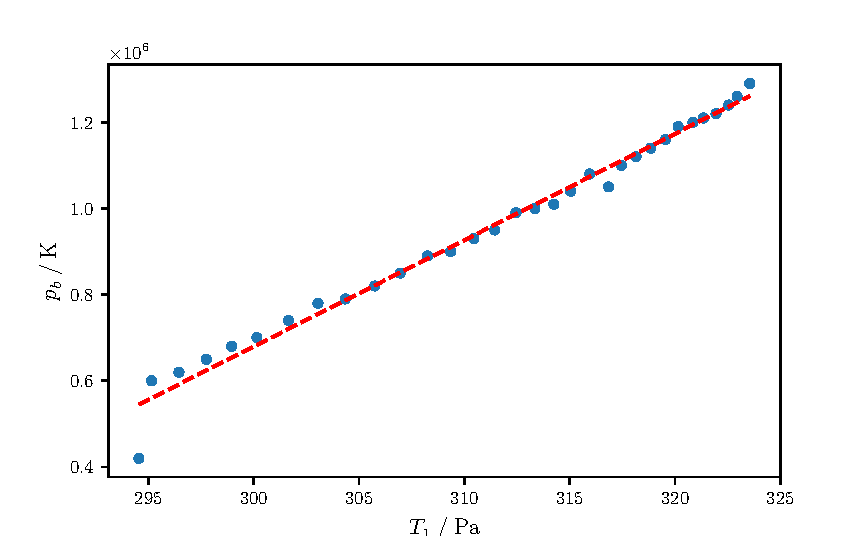
\includegraphics{Test.pdf}
  \caption{Temperatur und Druckverlauf}
  \label{fig:plot3}
\end{figure}



In \autoref{tab:massendurch3} ist der Massendurchsatz zu den vier gewählten Zeitpunkten dargestellt.
\begin{table}[H]
  \label{tab:massendurch3}
  \centering
  \sisetup{table-format=1.5}
  \begin{tabular}{S S}
    \toprule
    & {$\dfrac{\text{d}m}{\text{d}t}  \left[\unit{\dfrac{\kilogram}{\second}}\right]$}  \\
    \midrule
    {$t_1 = 380  \, \unit{\second}$} & {$8.0284 \pm 0.3799$}  \\
    {$t_2 = 760  \, \unit{\second}$} & {$6.6366 \pm 0.4451$}  \\
    {$t_3 = 1140 \, \unit{\second}$} & {$5.2447 \pm 0.5381$}  \\
    {$t_4 = 1520 \, \unit{\second}$} & {$3.8528 \pm 0.6470$}  \\
    \bottomrule
  \end{tabular}
  \caption{Massendurchsatz zu verschiedenen Zeitpunkten}
\end{table}

\subsection{Bestimmung der mechanischen Kompressorleistung}

Nach \eqref{eq:kompressorleistung} ergibt, wenn der Differenzenquotient erneut als Differenzialquotient geschrieben wird
\begin{equation}
N_{mech}= \dfrac{\text{d}A_m}{\text{d}t} = \dfrac{1}{κ-1} \left(p_b\left(\dfrac{p_a}{p_b}\right)^{\dfrac{1}{κ}}-p_a\right) \dfrac{\text{d}V_a}{\text{d}t} = 
    \dfrac{1}{κ-1} \left (p_b \left(\dfrac{p_a}{p_b} \right)^{\dfrac{1}{κ}}-p_a \right) \dfrac{1}{ρ}\dfrac{\text{d}m}{\text{d}t}.
\end{equation}
mit 

\begin{equation*}
\rho = \dfrac{\rho_0 T_0 p_a}{T_2 p_0}.
\end{equation*}

Es folgt die \autoref{tab:kompressorleistung2}

\begin{table}[H]
  \centering
  \label{tab:kompressorleistung2}
  \sisetup{table-format=1.4}
  \begin{tabular}{S S S}
    \toprule
    & {$\rho$}&{$N_{mech} \mathbin{/} \unit{\watt}$} \\
    \midrule
    {$t_1 = 380  \, \unit{\second}$} & {$0.0046 \pm 0.0001$} & {$ 8.0202 \pm 0.7682$} \\
    {$t_2 = 760  \, \unit{\second}$} & {$0.0053 \pm 0.0004$} & {$10.9729 \pm 1.2440$} \\
    {$t_3 = 1140 \, \unit{\second}$} & {$0.0060 \pm 0.0008$} & {$11.3432 \pm 1.7971$} \\
    {$t_4 = 1520 \, \unit{\second}$} & {$0.0066 \pm 0.0014$} & {$9.81943 \pm 2.3067$} \\
    \bottomrule
  \end{tabular}
  \caption{Die mechanische Kompressorleistung}
\end{table}

%\newpage

%\subsection{Sonstige Plots}
%
%In diesem Abschnitt befinden sich lediglich sonstige Plots, die der Vollständigkeit halber zwar enthalten sind, zur 
%Bestimmung vorangegangener Größen aber nicht von großer Bedeutung sind.

%3. Plot

%\begin{figure}
%  \centering
%  \includegraphics{plot_2.pdf}
%  \caption{Zeitlicher Druckverlauf in den Reservoiren.}
%  \label{fig:plot3}
%\end{figure}

%5. Plot

%\begin{figure}
%  \centering
%  \includegraphics{plot_5.pdf}
%  \caption{Zeitlicher Verlauf der Leistung.}
%  \label{fig:plot5}
%\end{figure}
